

\documentclass[conference]{IEEEtran}
\usepackage{blindtext, graphicx}
\usepackage{color}
\usepackage{scrextend}
\hyphenation{op-tical net-works semi-conduc-tor}


\begin{document}

\title{Paper Review}

\author{\IEEEauthorblockN{Yuting Cao}
\IEEEauthorblockA{University of South Florida\\
Email: cao2@mail.usf.edu}
}
\maketitle


\begin{abstract}
Briefly summarize all the papers I read about post silicon validation.
\end{abstract}


\section{probablisitic bus-masking analysis for post-silicon tests in microprocessor verification}
Provide an efficient, static bug-masking analysisi solution BugMAPI that tracks the information flow in a 
test program and estimates the probability that bugs go undetected by the checking mechanisms in place
in the post silicon platform.
This one I thought can b e used as heuristic for singal selection, but turned out to be helpful for test generator.

\section{Post-silicon validation of mulrtiprocessor memory consisitency~\cite{mammo2015post}}
monitor the system memory acccess information by changing a small portion of the l1 cache and an extra samll hardware logic.
The logged information will then be transfered to central memory to conduct analysis process.
The method used to detect memory error is by constructing a graph representation of memory interactions, an cycle indicates an error.

Compared to simulation based dynamic analysis, this is faster but less accurate.

Two limitations: lack of patches for mask-causing store instructions and false negatives in analysis.
System overview is shown in Figure.~\ref{systemoverview}
\begin{figure}
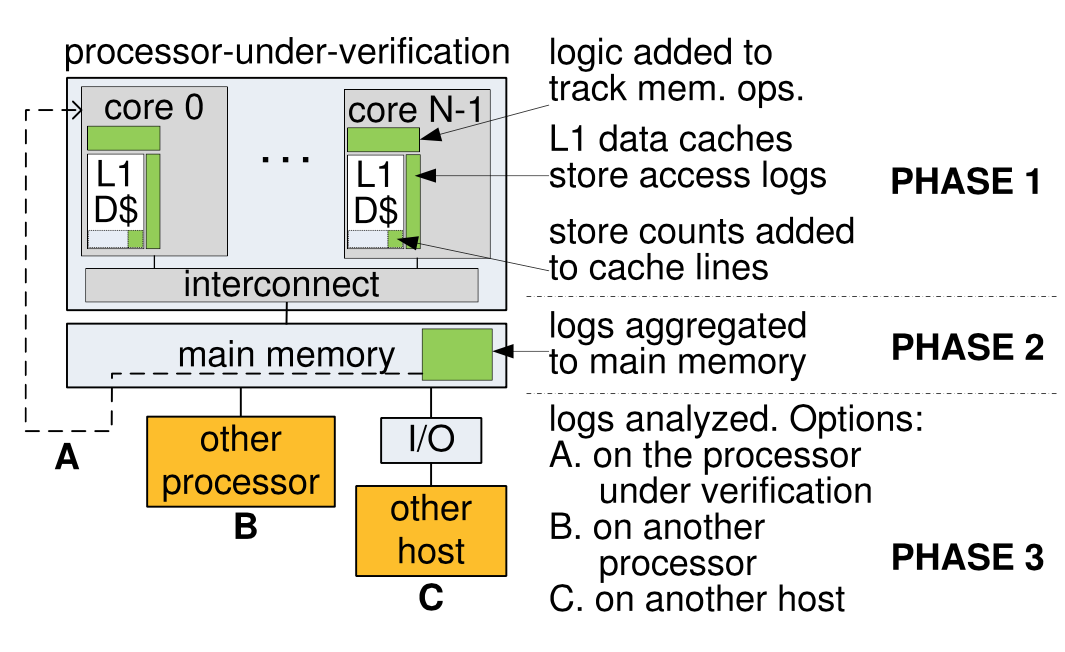
\includegraphics[width=0.5\textwidth]{systemoverview.png}
\caption{System Overview. Each core is modified to track memory accesses.
A portion of the L1 caches are temporarily reserved for logging memory accesses. A store counter is attached to each cache line to track the order of writes to the line. Finally, the analysis of the logged data is performed in software, which can be carried out on a processor/host available for the task.}
\label{systemoverview}
\end{figure}

\section{Cant See the Forest for the Trees: State Restoration?s Limitations in Post-silicon Trace Signal Selection ~\cite{forestMa}}
This paper proposed the the signal selection standard SSR(State Restoration Ratio) is not suitable for evaluating trace signal quality. It should be replaced by metric that allows good high-level behavioral coverage.

SRR measures the number of design states reconstructed from the signals observed. SRR= number of signals observed and restored / number of observed signals. The reason why SSR is not optimal is because 
\begin{itemize}
\item SRR treat all signals equally. but some signals are more important than others
\item SRR favors big arrays, which may not be useful for debugging at all
\end{itemize}

This paper proposed a new metric that is assertion coverage, as how many assertion are satisfied by the observed signals. The drawback it will introduce is the subjectivity and incompleteness. \(WHY??\)

This paper also introduced a new signal selection algorithm inspired from Google's PaperRank system. This algorithm is based on the connectivity of each instance, and by that find the most important signals. One thing is that it will avoid inclusion of entire array but select only relevant signals in stead. With experiment done with different test bench, it's proven that Paperbank algorithm allows much higher assertion coverage than SSR algorithm's selected signals.

One drawback of the Paperband algorithm is that it can't cover system-level assertions, because they don't trace interface signals. The phrase here is very odd, \"non of the algorithms are able to cover system level assertions, since they do not trace interface signals. This illustrates that optimizing for a functional coverage metric like assertion coverage will lead to interface signals being emphasized over internal signals. \" 	VERY CONFUSING.!!!!

CONCLUSION: This paper compared algorithm of Paperbank on netlist, PaperBank on RTL, SigSeT(SRR maximizing algorithm) with different metric including SRR, behavioral coverage, assertion coverage. The result shows that signal set with good SRR usually have less behavioral coverage and assertion coverage. The PaperBank on RTL model turns out to be the best algorithm for better debugging. 

I don't think this algorithm is fit for my research since there are not much attention on communication signals. 




\section{SYSTEM-LEVEL TRACE SIGNAL SELECTION FOR POST-SILICON DEBUG USING LINEAR PROGRAMMING}
This paper propose to automate trace signal selection instead of manual selection due to the increasing complexity of the system. It use the functional coverage as a metric and choose the low-level signals that produce a good coverage. And gradually refine the solution to allow the best behavioral coverage. 

This paper focus on the communications between IPs and try to maximize the coverage of each protocol messages.

The algorithm proposed in this paper is mainly protocol based.  As showed in ~\ref{procedure}, this algorithm 
\begin{itemize}
\item will first define a family of protocol in an understandable format. then decompose all messages in protocol into a messages contain only one data filed. 
\item For each Channel, form a set of messages that it covers
\item Using a linear program to find a set of signals to trace that allows the maximum frequency coverage. see Figure.~\ref{linear}
\item For high reward solutions, calculate heuristic intervals. See Figure.~\ref{interval}
\item Select best solution with small I/\(1+FC\) where I is interval score and FC is frequency coverage.
\end{itemize}

When find bugs and we want to refine the select signals to enable better root cause finding. There are several ways we can use.
\begin{itemize}
\item Block-Specific Views. For possible root cause blocks, assign messages in protocol family into each block and apply coverage-interval algorithm to them
\item Control View

As referred in Fig.~\ref{control}, we define all protocols and then find local and external decision points. Local decision points refers the messages with conditions. External decision point is messages that have same sender, data fields but different receiver. Calculating the advantage of the external decision point is NOT VERY CLEAR FOR ME YET. 
\end{itemize}


\begin{figure}[!ht]
\caption{Step-by-step flow of global view and block view selection method}
\label{procedure}
\centering
    \includegraphics[width=0.5\textwidth]{proc}
\end{figure}
\begin{figure}[!ht]

\caption{Linear Program Formulation}
\label{linear}
\centering
    \includegraphics[width=0.5\textwidth]{lin}
\end{figure}

\begin{figure}
\caption{Spacing example for a nine message sequence with four messages covered. Red circles indicate message is observable}
\label{interval}
\centering
    \includegraphics[width=0.5\textwidth]{inter}
\end{figure}


\begin{figure}
\caption{Step-by-step flow of control view selection method}
\label{control}
\centering
    \includegraphics[width=0.4\textwidth]{control}
\end{figure}




\section{On the cusp of a validation wall~\cite{validationWall}}
This paper goes through the definition of silicon validation and reason why it's important, together with the current techniques used for pre and post silicon validation.

Validation is the activity of ensuring a product satisfies its reference specifications, runs with relevant software and hardware, and meets user expectations.

Numbers of processor bug are growing for every new generation and the bugs are becoming more diverse and complex. which makes silicon testing even harder.

Effective validation needs
\begin{itemize}
\item modular validation (virtual platform) :

virtual platform helps find problems before post silicon validation, forcing the combination of pre and post silicon validation. And also enables early software development on the virtual platform.

Formal verification vs Dynamic verification
\item good analog and simulation.
\item test generator

To ensure all cases covered by test generator in stead of single area.
\item coverage measurement
\item assisted insertion of test
\item debugging features.
\end{itemize}

What I learned:
Post silicon validation is very complex and effort intensive compared to pre-silicon validation. Not very automated, which is needed in scholar field.


\section{Validation of SoC Firmware~Hardware Flows: Chanllenges and Solution Directions ~\cite{fw}}
\begin{itemize}
	\item Challenges of SoC firmware hardware flows
	\item specification error found late in product life-cycle.
		goal: analyze architecture specificaion
		methods: 1. executable specification written in programing language or formalism. (SystemC)
				question?paper said it?s not good because ?effort to develop executable specification is too high for adoption by the 						architecture team. "
				2. formal-specification language. (Proemela)

	\item stand alone FW or HW validation is problematic
		goal: co-validation. 
		methods: Do FW validation in the early stage by using a virtual platform of the HW as a development environment for FW. Start FW 			development simultaneously with HW development, to start the validation effort early.

	\item distribution of flows across many IPs and subsystem. Each flow has its own functionality.
		goal: need to separate concerns, allow better modularity in validation.
		methods: Design for verification
				(A little confused)
\end{itemize}

\section{Effective Post-Silicon Validation of System-on-Chips Using Quick Error Detection ~\cite{qed} }

{\color{red} reading: ref 9 about priori and 46 for algorithm about software signature and flow checking}
This paper introduced a method called Quick Error Detection (QED) for systematically creating test cases that can quickly detect bugs inside components.
The advantage of QED is it has a much shorter error detection latencies and increase the bug coverage.
The Fig.~\ref{fig1} shows the bug activation criteria and bug effects tables. Bug activation criteria is a set of conditions that mush be satisfied to activate a bug scenario. Bug effects is the resulting wrong behavior. Variable X, Y can be defined as any numbers with bound predefined.

 QED systematically transforms original tests into new QED tests families.  New tests will have bounded error detection latency.
 
 Methods: transformations:
 \begin{itemize}
 
 \item Error Detection Using Duplicated Instruction for Validation (EDDI-V)
 
 Bound error detection latency for bugs inside processor cores. Duplicate instructions and registers, and with same instruction, check if the corresponding value are same. If not, error find.
 
 \item PLC (for uncore components)
 
 Insert special PLC operations at very fine granularities across memory (and I/O) spaces using targeted instructions. It does self checking on selected set of variables .
 
 Compatible with EDDI-V
 
 \item CFCSS-V and CFTSS-V (for core's control flow)
 
 \begin{itemize}
 \item CFCSS-V
 
Checks the control flow of a test program during runtime against the control flow graph constructed during the test program?s compile time. Instead of checking between basic blocks, check between "blocks of instructions" that may contain arbitrary number of instructions (determined by $Inst\_min$ and $Inst\_max$) to balance trade offs between error detection latency and intrusiveness. Checking flow between every instruction will result in short error detection latency but increase the intrusiveness. While multiple blocks will lead to longer error detection latency.

Basic Idea: each block of instructions is assigned a unique integer as software signature. {\color{red} Detail need to be read from another paper. }
\item CFTSS-V
 see fig.~\ref{cftss} {\color{red} confused}
 \begin{figure}
 \caption{Pseudo assembly code for the CFTSS-V operation inserted at the beginning of each ?block of instructions.?}
\label{cftss}
\centering
    \includegraphics[width=0.4\textwidth]{cftss}
\end{figure}
\end{itemize}

\item Comparison of QED transformations in fig.~\ref{comp}
\begin{figure}
 \caption{COMPARISON OF QED TRANSFORMATIONS}
\label{comp}
\centering
    \includegraphics[width=0.4\textwidth]{comp}
\end{figure}
 \end{itemize}

\begin{figure}
\caption{bug activation criteria and bug effects}
\label{fig1}
\centering
    \includegraphics[width=0.4\textwidth]{bug}
\end{figure}



\section{A Common Platform for bridging Pre- and Post-Silicon Verification in Mixed-Signal Designed ~/cite{commonplatform}}
Motivation: majority of current verification is for digital or analog designs only. Great demand for new test technology to verify both digital and analog together. Physical bus increase due to the rising complexity of the interactions between analog and digital modules and smaller feature sizes.

Advantagement: allows simulation test case reusing for post-silicon verification. Development of a bidirectional bridging approach. It's generic, can be applied to a lot areas.

Concepts: 
\begin{itemize}
\item Exerciser runs on the DUV to create a simulator-like environment for post-si verification. Exerciser can generate test cases for pre-defined scenarios, run on target and auto checking. 
\item directed tests: predefined, written by hand
\item random tests: generated by transaction generators
\item direct random tests: hybrid
\end{itemize}

Method detaisl: 
\begin{itemize}
\item veication activities need to be planned ahead. (determine objectivies, how to achieve them. Done seperately for pre and post sili, \color{red}{may cause problems})
\item as showed in fig.~/ref{appr}
\item Test cases will be written in scripting language (pearl or python) to allow a high level abstractionand option to store and process data. Also allows for all 3 types of test cases generation
\item 
\end{itemize}

\begin{figure}
 \caption{Basic Concept of the Proposed Approach}
\label{appr}
\centering
    \includegraphics[width=0.5\textwidth]{appr}
\end{figure}


\section{Debugging Multi-Core System-on-Chip}
\begin{itemize}	
\item Introduction
		Design of an SOC: slowly decrease the abstraction level by level, adding details iteratively until it's ready for fabrication.
						  Each level the system will be verified using verification technique.
\item Why debug is difficult
	\begin{enumerate}
	\item Limited internal observability: data volume too big, can't be all recorded
	\item Asynchronicity and Consistent Global State: Different clock frequency between IPs
			globally-asynchronous locally synchronous design style: valid-accept handshake 
			global state sampled at greatest common divisor of frequencies
	\item Non-Determinism and Multiple Traces
			non determinism of shared slave create faulty traces
	\end{enumerate}			
\item Debugging an SoC
		3 types of errors:
		\begin {enumerate}
		\item Within a trace: permanent/transient error. (cause error for all following states )
		\item  Between traces: constant when occurs in every run (deterministic) / intermittent(non-deterministic)
		\item  Between systems: intrusive (changes the behavior of the system -probe effect)
		\item Debugging process:
			graph 5.9 b
		\end{enumerate}
\item Debug Methods
		Properties:
			\begin {enumerate}
			\item structural abstraction: which part of system to observe within one abstraction level, at what granularity
			\item temporal abstraction: what and how often we observe
			\item behavioral abstraction: what logical function is executed by a hw module
			\item data abstraction: how we interpret data
			scope is combination of structural and temporal abstraction
			\end{enumerate}
		Existing debug methods:
			\begin {enumerate}
			\item physical and optical debug: non-intrusive, lowest level of abstraction
			 	can only access wires close to the surface due to metal layers
			\item logical debug: built in support (design for debug DfD) to increase internal observability and controllability
			 	tradeoff b/w real-time behavior <-> amount of state inspected
			 	examples that address problems caused by asynchronicity, inconsistency of global states , non-determinism or multiple traces
					\begin {enumerate}
			 		\item Latch Divergence Analysis: running a cpu many times, compare right traces and wrong traces
			 			easily automated. doesn't distinguish noise in substate due to intermittent errors
			 		\item Deterministic Replay
			 			record non deterministic order and force deterministic
			 			A lot of specific method that I don't understand now
			 		\item Use of Abstraction for Debug
			 			distinguish b/w inter-process communication and intra-process computation. Allows filtering only useful info
					\end{enumerate}
			\item future research need
				debug method for parallel software and hw
			 \end{enumerate}	 	
\end{itemize}		
\ifCLASSOPTIONcaptionsoff
  \newpage
\fi


\bibliographystyle{IEEEtran}
\bibliography{bib}


\begin{IEEEbiography}[{\includegraphics[width=1in,height=1.25in,clip,keepaspectratio]{picture}}]{John Doe}
\blindtext
\end{IEEEbiography}
\end{document}


